	%You can delete all the comments after you have finished your document
%this sets up the defaults for the documents, 12pt font and A4 size. The article type sets this up as such as opposed to letter or memo.

%for the finer points LaTeX see https://en.wikibooks.org/wiki/LaTeX or http://tex.stackexchange.com/

\documentclass[12pt,a4paper]{article}
\usepackage{titlesec} %these are how we import packages, one helps set up footers and title layout
\setcounter{secnumdepth}{4}
\usepackage{fancyhdr}

% !TEX TS-program = pdflatex
% !TEX encoding = UTF-8 Unicode
\usepackage[utf8]{inputenc} % set input encoding (not needed with XeLaTeX)

\usepackage{graphicx} % support the \includegraphics command and options

\usepackage[parfill]{parskip} % Activate to begin paragraphs with an empty line rather than an indent

%%% PACKAGES
\usepackage{cite} % for IEEE style number references
\usepackage{setspace} % for control over line spacing
\onehalfspacing
\usepackage{booktabs} % for much better looking tables
\usepackage{array} % for better arrays (eg matrices) in maths
\usepackage{paralist} % very flexible & customisable lists (eg. enumerate/itemize, etc.)
\usepackage{verbatim} % adds environment for commenting out blocks of text & for better verbatim
\PassOptionsToPackage{hyphens}{url}\usepackage{hyperref} % adds \url command for hyperlinks in text, makes them black and allows wrapping on url hyphens
\hypersetup{
	colorlinks=false,
	linkcolor=black,
	filecolor=black,      
	urlcolor=black,
}
\usepackage{subfig} % make it possible to include more than one captioned figure/table in a single float
%\usepackage[authoryear]{natbib} % adds APA referencing style to standard LaTeX bibliography support
\usepackage[toc,page]{appendix}
% These packages are all incorporated in the memoir class to one degree or another...

%header and footer settings
\pagestyle{fancyplain}
\fancyhf{}
\renewcommand{\headrulewidth}{0.5pt}
\renewcommand{\footrulewidth}{0.5pt}
\setlength{\headheight}{15pt}
\fancyhead[L]{Beej Persson - 40183743}
\fancyhead[R]{SOC10101 Honours Project}
\fancyfoot[L]{}
\fancyfoot[C]{\thepage}

%set better section layout

\makeatletter
\renewcommand\paragraph{\@startsection {paragraph}{1}{0mm} % name, level, indent
	                           {3pt plus 2pt minus 1pt} % before skip
	                           {3pt plus 0pt} % after skip
	                           {\normalfont}}
\makeatother
\makeatletter
\renewcommand\subsubsection{\@startsection {subsubsection}{1}{0mm} % name, level, indent
	                           {3pt plus 2pt minus 1pt} % before skip
	                           {3pt plus 0pt} % after skip
	                           {\normalfont\bfseries}}
\makeatother
\makeatletter
\renewcommand\subsection{\@startsection {subsection}{1}{0mm} % name, level, indent
                               {3pt plus 2pt minus 1pt} % before skip
                               {3pt plus 0pt} % after skip
                               {\large\bfseries}}
\makeatother
\makeatletter
\renewcommand\section{\@startsection {section}{1}{0mm} % name, level, indent
                               {4pt plus 2pt minus 1pt} % before skip
                               {4pt plus 0pt} % after skip
                               {\Large\bfseries}}
\makeatother


%this starts the document
\begin{document}

%you can import other documents into your main one, these layout the Title and Declarations on its own page.
%you might need to change these to \ if your on Microsoft Windows.
\begin{singlespace}	
\newcommand{\HRule}{\rule{\linewidth}{0.5mm}}

\begin{titlepage}
	\begin{center}

	\HRule \\[0.4cm]
    	{\Large \bfseries Real-World Object Capture in a \\ Mixed Reality Environment\par}
	\vspace{0.2cm}
	\HRule \\[1.5cm]

	
    	\vspace{3cm}
	\begin{minipage}{0.4\textwidth}
	\begin{center} \large
        \emph{}\\
        	Beej Persson - 40183743
				
   	 \end{center}
    	\end{minipage}
	
	\vspace{2cm}
    	\begin{minipage}{1\textwidth}
    	\begin{center} \large
        
		Submitted in partial fulfilment of \\
		the requirements of Edinburgh Napier University \\
		for the Degree of \\
        	BSc (Hons) Games Development
    	\end{center}
    	\end{minipage}

    	\vfill

    	% Bottom of the page
	\begin{minipage}{1\textwidth}
    	\begin{center} \large
		School of Computing
    	\end{center}
    	\end{minipage}
	
	\vspace{1cm}
    	{\large \today}


	\end{center}
\end{titlepage}
%{\large Submitted in partial fulfilment of the requirements of Edinburgh Napier University for the Degree of }

\section*{Authorship Declaration}
\vspace{0.5cm}
\begin{flushleft}
I, Beej Persson, confirm that this dissertation and the work presented in it are my own achievement.\newline

Where I have consulted the published work of others this is always clearly attributed;\newline

Where I have quoted from the work of others the source is always given. With the exception of such quotations this dissertation is entirely my own work;\newline

I have acknowledged all main sources of help; \newline

If my research follows on from previous work or is part of a larger collaborative research project I have made clear exactly what was done by others and what I have contributed myself;\newline

I have read and understand the penalties associated with Academic Misconduct.\newline

I also confirm that I have obtained informed consent from all people I have involved in the work in this dissertation following the School's ethical guidelines.\newline
\end{flushleft}

\begin{flushleft} \large
\emph{Signed:} \\
\end{flushleft}

\vspace{.5cm}

\begin{flushleft} \large
\emph{Date:} \\
\end{flushleft}

\vspace{.5cm}

\begin{flushleft} \large
\emph{Matriculation no: }  \\
\end{flushleft}
\pagebreak

\section*{Data Protection Declaration}
\vspace{0.5cm}
\begin{flushleft}
Under the 1998 Data Protection Act, The University cannot disclose your grade to an unauthorised person. However, other students benefit from studying dissertations that have their grades attached. \newline

\vspace{0.5cm}

Please sign your name below one of the options below to state your preference.\newline
\vspace{0.5cm}

The University may make this dissertation, with indicative grade, available to others.\newline
\vspace{3cm}


The University may make this dissertation available to others, but the grade may not be disclosed.\newline
\vspace{3cm}


The University may not make this dissertation available to others.\newline
\end{flushleft}


\pagebreak

%LaTeX let you define the abstract separately so it wont get sucked into the main document.
\begin{abstract}
% fill the abstract in here
\end{abstract}
\pagebreak
\setcounter{tocdepth}{2}
\tableofcontents % is generated for you
\newpage

\listoftables
%generated in same way as figures
\newpage

\listoffigures
%you may have captions such as equations, listings etc they should all appear as required
%these are done for you as long as you use \begin{figure}[placement settings] .. bla bla ... \end{figure}
\newpage

\section*{Acknowledgements}
Insert acknowledgements here
\subsection*{}
	I would like to thank my widely-desired work ethic, talk-of-the-town dedication and my optimistic opinions of my abilities.
\end{singlespace}
\newpage


\section{Introduction}
\subsection{Background}
This project has three main background components to discuss. These are mixed reality, the Microsoft HoloLens and Vuforia.

\subsubsection{Mixed Reality}
\paragraph{Virtual Continuum}
Mixed reality (MR) is a variation of virtual environments, or virtual reality. A virtual environment is one in which a user is immersed inside a synthetic environment. Whilst in this environment the user cannot see the real world around them, what they see is entirely virtual. In a mixed reality environment, however, the user is able to see aspects of both the real world and super-imposed virtual objects. MR "supplements reality, rather than completely replacing it" \cite{azuma97}.

\begin{figure}[!h]
	\centering
	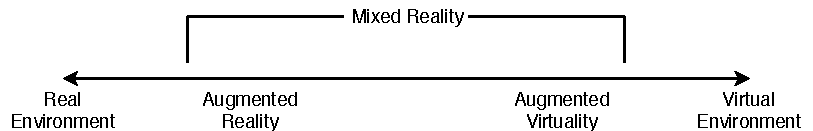
\includegraphics[width=\textwidth]{images/virtualitycontinuum}
	\caption{The Virtuality Continuum}
	\label{fig_mr}
\end{figure}

MR is often considered as encompassing both augmented reality (AR) and augmented virtuality (AV), both of which reside along the "virtuality continuum" (see Figure \ref{fig_mr}), a term coined by Milgram and Kishino in 1994  \cite{milgram94}, with the real world at one end and the virtual at the other. AR refers to an otherwise real world environment in which there can be seen virtual augmentations, often viewed through a clear screen. AV, conversely, attempts to merge real world scenery or objects into an otherwise virtual world.

\paragraph{Applications and Devices}
The nature of combining real and virtual objects can be utilised in a variety of ways and can enhance a user's ability to perform certain tasks and interact with the world. Whilst initially prevalent in the arts and entertainment industries, MR has a number of practical uses and is being taken advantage of by businesses today, particularly in the fields of military training, manufacturing and education \cite{evans17, hughes97}. Many devices utilise these virtual environments, such as the Oculus Rift and the HTC Vive, headsets that need to be connected to a computer or console, both released in 2016, but the Microsoft HoloLens is one of the few standalone devices available that offers mixed reality capabilities in a head-mounted display.

\subsubsection{Microsoft HoloLens}
The Microsoft HoloLens is a mixed reality holographic head-mounted display unit with an adjustable cushioned headband released in 2016 \cite{microsoftcorp}. It is "the first fully untethered holographic computer running Windows 10", enabling a mixed reality experience with no wires, no external cameras and no connection to a PC required \cite{holmdahl15}.

\paragraph{Hardware, Sensors and Features}
\begin{table}[!h]
	\renewcommand{\arraystretch}{1.3}
	\caption{Microsoft HoloLens Hardware Specifications}
	\label{hardware}
	\centering
	\begin{tabular}{l|l}
		\toprule
		CPU & Intel Atom x5-Z8100 @ 1.04GHz\\ \hline
		GPU/HPU & HoloLens Processing Unit \\ \hline
		RAM & 2.0GB\\ \hline
		Storage & 64GB\\ \hline
		OS & Windows 10 32-bit\\ \bottomrule
	\end{tabular}
\end{table}
The optics are two separate displays, which are viewed through glass lenses, on to which images are projected and layered to produced what the user can see in their space. The HoloLens' system is essentially mobile hardware (see Table \ref{hardware}) featuring an Intel Cherry Trail Atom chip \cite{rubino16}. Additionally, however, it runs a few processors that make it unique. There is an inertial measurement unit (IMU), which includes an accelerometer, gyroscope, and magnetometer, and there is an aptly named Holographic Processing Unit (HPU), that handles where the user is looking, gesture tracking, spacial mapping and more. \cite{holmdahl15}.

It has four "environment understanding cameras", two on each side, which provide the basis for tracking the user's head; a depth camera, which helps with hand tracking and performs surface reconstruction (for placing holograms on physical objects); a video camera and an ambient light sensor. These sensors work with the optics module and the IMU and is packaged for the Intel Atom chip by the HPU to produce fast response times to movement so that the user's position is updated and displayed in less than 10ms to ensure the holograms feel part of the world. The HoloLens also features four microphones for receiving user commands, mounted stereo speakers providing spatial sound and both WiFi and bluetooth \cite{colaner16}.

\paragraph{Practical Applications}
As of 2018 there has only been a few practical applications of the Microsoft HoloLens and a number of them have only been proof of concepts so far. Notably there has been a number of applications developed by NASA in partnership with Microsoft. In 2015 they teamed up for the OnSight and Sidekick projects, utilising the HoloLens on the International Space Station for communication and real-time guidance with ground operators, and later again in 2017 to help find the best places on Mars to build bases \cite{nasa15, microsoftnews17}.

There are also a couple of examples of use in medicine. In 2017 a team of surgeons used the HoloLens to visualise MRI and radiography information whilst operating on a patient with a malignant tumour patient \cite{bernardo17, 3ders17}. Also in 2017 an ultrasound training simulation was designed to teach healthcare workers proficiency in anatomy through interaction with 3D holograms of internal human structures \cite{lynn17, mahmood17}.

Microsoft are also working on using the HoloLens as a means of communication as part of a research project called Holoportation \cite{cutler17}. Users will have high quality 3D models of themselves rendered in each other's local space. The goal is to allow them to see, hear and interact with one another as if they were in the same room \cite{orts16}.

There have been even fewer examples of applications that make use of Vuforia's tracking capabilities to build interactive experiences. In 2017 a simple proof of concept assembly instruction application was attempted in Unity that featured user interfaces, dynamic 3D assembly instructions and spatially registered content placement \cite{evans17}.

\subsubsection{Vuforia}
Vuforia is an augmented reality software development kit designed for Android, iOS and Universal Windows Platform applications with support for phones, tablets and eyewear \cite{vuforia, vuforiaeyewear}. The Vuforia engine is natively integrated with the latest versions of Unity and provides the technology to recognise and track images and simple 3D objects in real time. Vuforia has a developer portal that allows for easy access to the SDK and associated tools, such as the Target Manager.

\paragraph{Target Manager}
The Vuforia Target Manager is a tool that allows the creation and management of target databases via the Vuforia developer portal. The databases can be assigned license keys by developers and enables easy management of the targets needed for separate applications. When creating applications users can choose which databases the SDK will use when attempted to detect targets. The tool can also be used to create new targets by uploading images and 3D models to the database and manipulating them to be in-line with the required format for specific targets \cite{vuforiatargetmanager}. 

\paragraph{Image Targets}

\begin{figure}[!h]
	\centering
	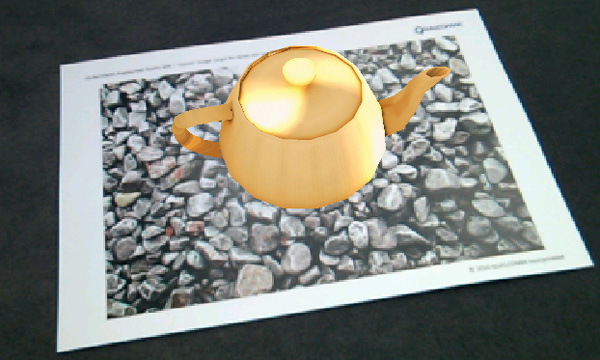
\includegraphics[width=10cm,height=10cm,keepaspectratio]{images/imagetarget}
	\caption{An Example Image Target}
	\label{fig_imagetarget}
\end{figure}

Image targets are flat images, such as printed media, that the Vuforia SDK can detect and track. They do not require special black and white spaces or codes to be recognised but instead the SDK tracks features that are found in the image itself by comparing those features against its target resource database. Once initially detected the SDK will continue to track the target whilst at least partially in the device camera's field of view and can perform an action or link virtual content to the target, such as the 3D rendered teapot that can be seen in Figure \ref{fig_imagetarget} (image retrieved from Vuforia's image target guide \cite{vuforiaimagetargets}).

\paragraph{Multi-Targets}
Multi-targets are created by combining multiple image targets and arranging them into a simple 3D geometric shape, such as a cube. All the faces of a multi-target can be tracked simultaneously as they possess a pre-defined position relative to the target's origin. As a result the entire object can be tracked when any one of its images has been detected  \cite{vuforiamultitargets}. These targets are created by defining a relationship between pre-existing image targets using the Vuforia Target Manager.

\paragraph{Object Recognition}
Object recognition allows the detecting and tracking of more intricate 3D objects by creating object targets made using the Vuforia Object Scanner. The object scanner, which only officially is supported on the latest Samsung Galaxy devices but can be configured to work on other Android devices \cite{vuforiasupportedversions}, is an application that can be used to scan a physical 3D object and produces an Object Data (*.OD) file and allows a visualisation of the object target and its coverage. The *.OD file produced by the application can then be uploaded to produce Vuforia's target manager and an object target to be produced \cite{vuforiaobjectreco}. The SDK will then be able to recognise the real-world object that was scanned by comparing it with the digital representation of the features and geometry that is provided by the object target.

\paragraph{VuMark}

\begin{figure}[!h]
	\centering
	\includegraphics[width=10cm,height=10cm,keepaspectratio]{images/examplevumarks}
	\caption{Example VuMarks}
	\label{fig_vumark}
\end{figure}

VuMarks are customised markers that encode data and support unique identification and tracking. They are similar to image targets in that they are 2D targets that can be detected and tracked, but provide a lot more than image targets cannot. As the same VuMark design can be used to encode a range of unique IDs or data, they enable the SDK to distinguish between identical looking products using their unique instance ID. VuMarks are designed to enable companies to create AR targets that subtly integrate with their brand, as shown in the example VuMarks in Figure \ref{fig_vumark} (image retrieved from Vuforia's VuMark guide \cite{vuforiavumark}). VuMarks are created using Vuforia's VuMark designer tool and then uploaded to the Vuforia Target Manager.

\paragraph{Model Targets}
Model targets enable physical objects to be detected and tracked using a 3D model of the object. The real-world objects are recognised by the Vuforia SDK using a "specially prepared target database that is generated by processing a digital 3D representation of the object" using the Model Target Generator tool. Supported objects must be rigid and have matte surfaces. For this to work, the 3D representation of the object should be accurate to a high degree of precision to the physical object. Vuforia's model target test application features a model that is to be 3D printed to be recognised by the SDK \cite{vuforiamodeltargets}.

\subsubsection{Summary of Findings}
Attempting to capture and manipulate real-world objects on the Microsoft HoloLens is mostly unexplored territory. The HoloLens provides spatial recognition hardware and sensors that allow for head and hand tracking but no built-in object recognition. Vuforia provides the tools to recognise real world objects through the use of a variety of targets stored in the online target databases. The SDK is integrated into Unity and supports development of Universal Windows Applications, as well as specifically stating support of the Microsoft HoloLens. 

\subsection{Aims and Objectives}
The aim of this project is to evaluate the effectiveness of real-world object capture and real-time object manipulation in a mixed reality environment using Vuforia on the Microsoft HoloLens. The goal will be to develop a method to recognise and track a simple 3D object in space using Vuforia's SDK. If a simple object is successfully detected and tracked then the scope of the project can extend to attempts at manipulation of the object and the capture of multiple and/or more complex objects. The manipulation attempts will include over-laying post-processing effects by applying shaders to the captured object to, for example, make it appear in greyscale or blurred. Further testing can be done to explore to what extent these manipulations can be performed in real-time given the limiting hardware of the HoloLens.

\subsubsection{Overview Of Milestones}
The objectives of this project can be summarised in these milestones:
\begin{itemize}\itemsep0pt
	\item simple physical object detection on the HoloLens
	\item simple object manipulation through the use of post-processing shaders
	\item complex, or multiple, physical objects detected simultaneously
	\item real-time object manipulation
\end{itemize}
And, if possible given the scope of the project:
\begin{itemize}\itemsep0pt
	\item multiple real-time manipulations of multiple detected objects
	\item determining the limits of the HoloLens hardware for real-world object manipulation
\end{itemize}

\subsection{Scope and Limitations}
\subsubsection{Scope}
The scope of the project is to work with the Vuforia SDK and build a Universal Windows Platform application in the Unity engine that runs on the Microsoft HoloLens. The application, if successfully implemented, should allow a user to detect, track and manipulate objects via a simple user-interface.

\paragraph{Main Deliverables}
The main deliverables of the project are listed below:
\begin{itemize}\itemsep0pt
	\item Object capture and manipulation implementation
	\item Full report of the project detailing the methodology followed, the implementation specifications and an evaluation of the work done
	\item Poster summarising the key features of the project
\end{itemize}

\paragraph{Importance of the Project}
Mixed reality is an emerging technology that can enhance a user's ability to interact with the world. An application that allows for detection and manipulation of real-world objects is one that can provide new ways to educate students, build virtual structures or even tell immersive stories. The project could benefit technical developers looking for innovative game mechanics or mixed reality enthusiasts seeking an immersive challenge.

\subsubsection{Limitations}
Vuforia's support of the Microsoft HoloLens is relatively unexplored. Certain features Vuforia offers may not all work with the HoloLens' specific hardware. Due to the nature of the relative niche that Vuforia's SDK seeks to fill, online forums and troubleshooting answers are scarce, especially when working primarily with the HoloLens.

\subsection{Structure of this Dissertation}
This dissertation is split into five primary chapters.

The first chapter seeks to provide a background to the technologies utilised by the project as well as an overview of the project's aims and scope. The second chapter details the methodology followed and how that affected the outcome of the project. The third chapter is a look at the specifics of what is provided in the application's implementation. The fourth chapter is an evaluation of the application, its relation to the initial goals and a discussion of whether the project was successful. The final chapter provides a conclusion to the dissertation that summarises the findings of the project as well as any future work this project can stand to benefit from. This section also includes a reflection on me, the author, and my feelings about the project.

\newpage
\section{Methodology}
\subsection{Getting to grips with Vuforia}
\subsubsection{Vuforia's Samples}
\subsection{Object Recognition}
\subsubsection{Choice Over Model Targets}
\subsubsection{Vuforia Object Scanner}
\subsection{Multi-Target}
\subsubsection {Changing Environment}
\subsection{Image Target}

\section{Implementation}
\subsection{Object Recognition}
\subsection{Multi-Target}

\section{Evaluation}

\section{Conclusion}
\subsection{Has the Project met its Aims?}
\subsection{Future Work}
\subsection{Personal Reflection}
\newpage
\begin{singlespace}	
\bibliographystyle{IEEEtran}
\bibliography{Bibliography}
\end{singlespace}

%example of References. See https://en.wikibooks.org/wiki/LaTeX/Bibliography_Management
%might be good to use a separate document for these so your main work is not one really long text file. 

%you can crate this on a extra tex document just like the title or any other part of the document.
\newpage
\begin{appendices}
\section{Initial Project Overview}
 \ \\ \textbf{SOC10101 Honours Project (40 Credits)} \\ \\
\textbf{Title of Project:} \\
Real world object-capture in a mixed-reality environment. \\ \\
\textbf{Overview of Project Content and Milestones:} \\
This project will look to evaluate the effectiveness of capturing real world objects using Vuforia on the Microsoft HoloLens. Initially, a method to capture a simple object will be developed, before attempts to capture more complex (or multiple) objects and real-time object manipulation will be implemented. The project aims to explore to what extent this can be done. \\
The milestones will be: 
\begin{itemize}\itemsep0pt
	\item simple object capture
	\item simple object manipulation
	\item complex object capture
	\item real-time object manipulation.
\end{itemize}
\textbf{The Main Deliverable(s):} \\
Object capture and manipulation software. \\
Dissertation. \\
Poster. \\ \\
\textbf{The Target Audience for the Deliverable(s):} \\
Technical mixed-reality game developers looking for new game mechanics. \\
Enthusiasts interested in new game technologies. \\ \\
\textbf{The Work to be Undertaken:} \\
Research similar attempts at mixed-reality object manipulation. \\
Design a method to capture a cube (or similar object) using Vuforia. \\
Build and apply simple shaders to the object. \\
Expand on above methods to capture more complex objects. \\
Explore and evaluate the extent to which the objects can be manipulated in real-time. \\
Document and report findings. \\ \\
\textbf{Additional Information / Knowledge Required:} \\
Creating and managing Unity projects. \\
How to use Vuforia. \\
Improve understanding of shader usage. \\ \\
\textbf{Information Sources that Provide a Context for the Project:} \\
General Development Page for the HoloLens: \\
\url{https://developer.microsoft.com/en-us/windows/mixed-reality/development} \\
Some related downloadable tools: \\
\url{https://developer.microsoft.com/en-us/windows/mixed-reality/install_the_tools} \\
Vuforia Specific: \\
\url{https://developer.microsoft.com/en-us/windows/mixed-reality/vuforia_development_overview} \\
\url{https://developer.vuforia.com} \\ \\
\textbf{The Importance of the Project:} \\
Mixed-reality is an emerging games technology with great potential for immersive story-telling and innovative game design. This project looks to explore an aspect of that and if successful could be beneficial to those interested in designing such games. \\ \\
\textbf{The Key Challenge(s) to be Overcome:} \\
Lack of similar projects documented. \\
Fairly niche/specialist/obscure software, mostly new territory. \\
\newpage

\section{Report on the Interim Review Meeting}
\ \\ \textbf{SOC10101 Honours Project (40 Credits)} \\                   
\textbf{Week 9 Report} \\ \\
\textbf{Student Name:} Beej Persson \\
\textbf{Supervisor:} Kevin Chalmers \\
\textbf{Second Marker:}  Gregory Leplatre \\
\textbf{Date of Meeting:}  20/11/2017 \\
Can the student provide evidence of attending supervision meetings by means of project diary sheets or other equivalent mechanism?  \textbf{no*} \\
\indent If not, please comment on any reasons presented \\
\textsl{No evidence provided but no indication from supervisor that there was a problem with weekly meeting attendance.} \\ \\ \\
Please comment on the progress made so far \\ \\
\textsl{The work done focused on identifying ways of working with a Hololens, i.e., the output side of the project. This was useful, but the main challenge of the project is object recognition and augmentation, which would have been useful to deal with earlier. This would also have allowed you to engage with relevant literature on the subject.} \\ \\ \\
Is the progress satisfactory? \textbf{unsure} \\
Can the student articulate their aims and objectives? \textbf{Partly} \\
If yes then please comment on them, otherwise write down your suggestions. \\ \\
\textsl{The overall goal (altering the appearance of real-world objects using AR) is clear. What specific alterations, to which objects and in which context remains to be determined. Familiarity with relevant literature will help you specify your project more accurately. Many things are possible, some more complex than others. For this type of project, a good approach would be to consider what operation would have the highest visual impact while having a manageable development cost. There is definitely potential in your project.} \\ \\ \\	
Does the student have a plan of work? \textbf{Yes} \\
If yes then please comment on that plan otherwise write down your suggestions. \\ \\
\textsl{Unfortunately, the plan is limited to work already done.} \\ \\ \\
Does the student know how they are going to evaluate their work? \textbf{partly} \\
If yes then please comment otherwise write down your suggestions. \\ \\
\textsl{The proposed approach is sensible but it is difficult to be more specific at this stage as the functionalities of the system aren’t clearly defined.} \\ \\
Any other recommendations as to the future direction of the project \\ \\
\textsl{With Vuforia, you should be able to capture objects in a scene (in advance) and then track these objects. The acquisition/tracking effectiveness probably depends on the complexity of the object, which you should establish. Once you know the limits of what you will be able to track, you can focus on real-time alterations. Your incremental development approach is suitable, but it needs to be better controlled. Once you know what you are aiming to do, you can define the incremental steps that will lead you there. The core of the research in this area is about achieving realism, which involves lighting and material acquisition. Potentially impactful results can also be achieved by taking slighting different directions. Giving an object a stylised look is one of them. Anecdotally, magic tricks are high impact and can be technically cheap. A magic trick you could implement could be: give a physical object to a user (that you will have previously scanned with Vuforia). Ask them to put it on a table (that you have also previously scanned), and make the object disappear (assuming the user is wearing a Hololens).} \\ \\
\begin{tabbing}
	Signatures: \hspace{1em} \= Supervisor \hspace{2em} \= Kevin Chalmers \\
	\> Second Marker \> Gregory Laplatre \\ \\
	\> Student \>
\end{tabbing}
Please give the student a photocopy of this form immediately after the review meeting; the original should be lodged in the School Office with Leanne Clyde
\newpage


\section{Diary Sheets (or other project management evidence)}
Insert diary sheets here together with any project management plan you have

\section{Appendix 4 and following}
insert content here and for each of the other appendices, the title may be just on a page by itself, the pages of the appendices are not numbered, unless an included document such as a user manual or design document is itself pager numbered.
\end{appendices}

\end{document}
